%==========================================================
% Roamly · Entrega 2: Descrição
% Compilar a partir desta pasta:  latexmk -pdf main.tex
% Estrutura: enunciado «Deliverable 2 | Description | 2026»
%==========================================================
\documentclass[11pt,a4paper]{article}

\usepackage[utf8]{inputenc}
\usepackage[T1]{fontenc}
\usepackage[portuguese]{babel}
\usepackage{lmodern}
\usepackage[margin=2.4cm]{geometry}
\usepackage{graphicx}
\usepackage{pdfpages}
\usepackage{pdflscape}
\usepackage{tabularx,longtable,booktabs,array,multirow}
\usepackage{enumitem}
\usepackage[table]{xcolor}
\usepackage{tcolorbox}
\usepackage{textcomp}
\usepackage{float}
\usepackage{caption}
\usepackage{subcaption}
\usepackage[nottoc]{tocbibind}
\usepackage[titletoc,title]{appendix}
\usepackage{fancyhdr}
\usepackage{docmute}   % \input de documentos completos (casos de uso) sem o seu preâmbulo
\usepackage{fvextra}   % \VerbatimInput dos ficheiros .feature (cenários BDD), com quebra de linha
\usepackage{hyperref}
\tcbuselibrary{breakable, skins}

%---------------------------------------------------------- dados do documento
\newcommand{\projeto}{Roamly - Wander\&Travel}
\newcommand{\entrega}{Entrega 2: Descrição}
\newcommand{\uc}{Requisitos e Especificações 2026}
\newcommand{\versao}{1.0}
\newcommand{\local}{Coimbra}
% mês e ano da compilação, em português (ex.: «novembro de 2026»)
\newcommand{\mesano}{\ifcase\month\or janeiro\or fevereiro\or março\or abril\or maio\or junho\or julho\or agosto\or setembro\or outubro\or novembro\or dezembro\fi\ de \the\year}
\newcommand{\equipa}{%
  \begin{tabular}{lll}
  Tiago Silva      & n.º 2022216215 & \texttt{tds@student.uc.pt} \\
  Gonçalo Ferreira & n.º 2022210563 & \texttt{uc2022210563@student.uc.pt} \\
  José Santos      & n.º 2022227876 & \texttt{uc2022227876@student.uc.pt} \\
  João Coelho      & n.º 2021275030 & \texttt{uc2021275030@student.uc.pt}
  \end{tabular}}

%---------------------------------------------------------- caminhos
% figuras e tabelas das outras pastas da 2.ª entrega (story_map/, diagrams/, ...)
\graphicspath{{../}}

%---------------------------------------------------------- estilo
\definecolor{roamly}{HTML}{0E6E68}
\definecolor{alerta}{HTML}{B3261E}
\definecolor{pendente}{HTML}{6B7280}
\hypersetup{colorlinks=true,linkcolor=roamly,urlcolor=roamly,citecolor=roamly,
  pdftitle={Roamly - Entrega 2: Descrição}}

\newcolumntype{L}{>{\raggedright\arraybackslash}X}
\renewcommand{\arraystretch}{1.3}
\setlist{nosep,leftmargin=*}
\captionsetup{font=small,labelfont=bf}

% referência a um registo de entrevista ou a um breakdown da Entrega 1
\newcommand{\reg}[1]{{\footnotesize\textcolor{pendente}{(#1)}}}
% casos de uso (os ficheiros de ../casos_de_uso/corrigidos/ usam estas macros; aqui cada um é uma subsubsecção)
\newenvironment{usecase}[2]{\subsubsection{#1: #2}\small\noindent\ignorespaces}{\par\medskip}
\newcommand{\ucField}[2]{\textbf{#1} & #2 \\}

\pagestyle{fancy}
\fancyhf{}
\fancyhead[L]{\small\projeto}
\fancyhead[R]{\small\entrega}
\fancyfoot[C]{\small\thepage}
\renewcommand{\headrulewidth}{0.4pt}

%==========================================================

\begin{document}

%---------------------------------------------------------- capa (sem número de página)
\begin{titlepage}
\centering

\includegraphics[width=0.7\textwidth]{figuras/logo_preto_uc_dei.pdf}\\[3cm]
{\color{roamly}\rule{\textwidth}{1.2pt}}\\[1.2em]
{\Huge\bfseries\color{roamly} \projeto}\\[0.6em]
{\LARGE\bfseries \entrega}\\[0.4em]
{\color{roamly}\rule{\textwidth}{1.2pt}}\\[3em]

{\large \uc}\\[3em]

{\large\bfseries Autores}\\[0.6em]
{\large \equipa}\\

\vfill
{\large \local, \mesano}\\[0.4em]
{\small Versão \versao}
\end{titlepage}


\tableofcontents
\listoffigures
\listoftables
\clearpage

%==========================================================
% No enunciado, a introdução não é numerada: o brief é a Secção 1.
\section*{Introdução}\label{sec:introducao}
\addcontentsline{toc}{section}{Introdução}

\subsection*{O projeto \projeto}

O \projeto{} é um agente de viagens baseado em inteligência artificial,
pensado, numa primeira fase, para jovens com orçamentos limitados
mas posteriormente para qualquer utilizador que queira simplificar o processo de planeamento de viagens.
Ainda pretendemos avaliar o potencial do \projeto{} em atender às novas necessidades de agências de viagens já
inseridas no mercado.

Na Entrega~1 estudámos como esse trabalho é feito hoje, com duas entrevistas contextuais: um jovem que organizou uma
viagem de grupo e um agente de viagens de balcão. Os modelos de trabalho mostraram que o problema não é só encontrar
opções baratas, mas saber quanto a viagem custa de facto, coordenar o grupo e o dinheiro e confiar no que a IA sugere.
Por isso a nossa visão deixou de ser um agente que propõe o itinerário sozinho e passou a ser um quadro que o
utilizador monta e que a IA vigia. Nesta entrega, o \projeto{} também não faz reservas nem processa pagamentos: o
organizador escolhe a proposta combinada e reserva no site de cada fornecedor.

Esta entrega descreve o sistema a construir a partir desses resultados.

\subsection*{Contexto}

Este projeto foi desenvolvido na unidade curricular de \uc{}, no Mestrado em Engenharia Informática do DEI da Universidade de Coimbra.
Não há um cliente externo: a ideia do \projeto{} partiu da equipa. Por isso, o \textit{brief} (Secção~\ref{sec:brief}) é a
ideia inicial com que a equipa propôs o projeto.

\subsection*{Estrutura do documento}

A Secção~\ref{sec:brief} apresenta o \textit{brief}. A Secção~\ref{sec:storymap} contém o \textit{story map} e as histórias de
utilizador. A Secção~\ref{sec:casosdeuso} apresenta o diagrama de contexto, o diagrama de casos de uso, os três casos de uso
detalhados e uma reflexão sobre um caso de uso gerado por IA. A Secção~\ref{sec:bdd} contém os cenários BDD, a
Secção~\ref{sec:ddd} o modelo de domínio, a Secção~\ref{sec:reflexao} a reflexão sobre o uso de IA e a
Secção~\ref{sec:conclusao} as conclusões.

%==========================================================
\section{O \textit{brief}}\label{sec:brief}

Não há cliente externo, por isso o \textit{brief} é a ideia com que a equipa propôs o projeto, antes de qualquer
investigação contextual. Fica aqui como foi formulada, ainda vaga e centrada na solução.

\begin{tcolorbox}[colback=roamly!6,colframe=roamly,arc=2pt,boxrule=0.8pt]
O \projeto{} é um agente de viagens baseado em inteligência artificial, pensado, numa primeira fase, para jovens com
orçamentos limitados e, mais tarde, para qualquer pessoa que queira simplificar o planeamento de uma viagem. As plataformas
atuais estão fragmentadas: obrigam a escolher primeiro um destino e a pesquisar à parte voos, alojamento e atividades.
O \projeto{} combina estas opções automaticamente, a partir do orçamento, das datas, dos interesses e da flexibilidade de
cada pessoa, e propõe um itinerário personalizado e acessível. Queremos também avaliar se pode responder às necessidades
das agências de viagens.
\end{tcolorbox}

%==========================================================
% O título fica na página deitada, junto do mapa, para não ficar sozinho no fim da página anterior.
\begin{landscape}
\section{\textit{Story map}}\label{sec:storymap}

\begin{figure}[H]
\centering
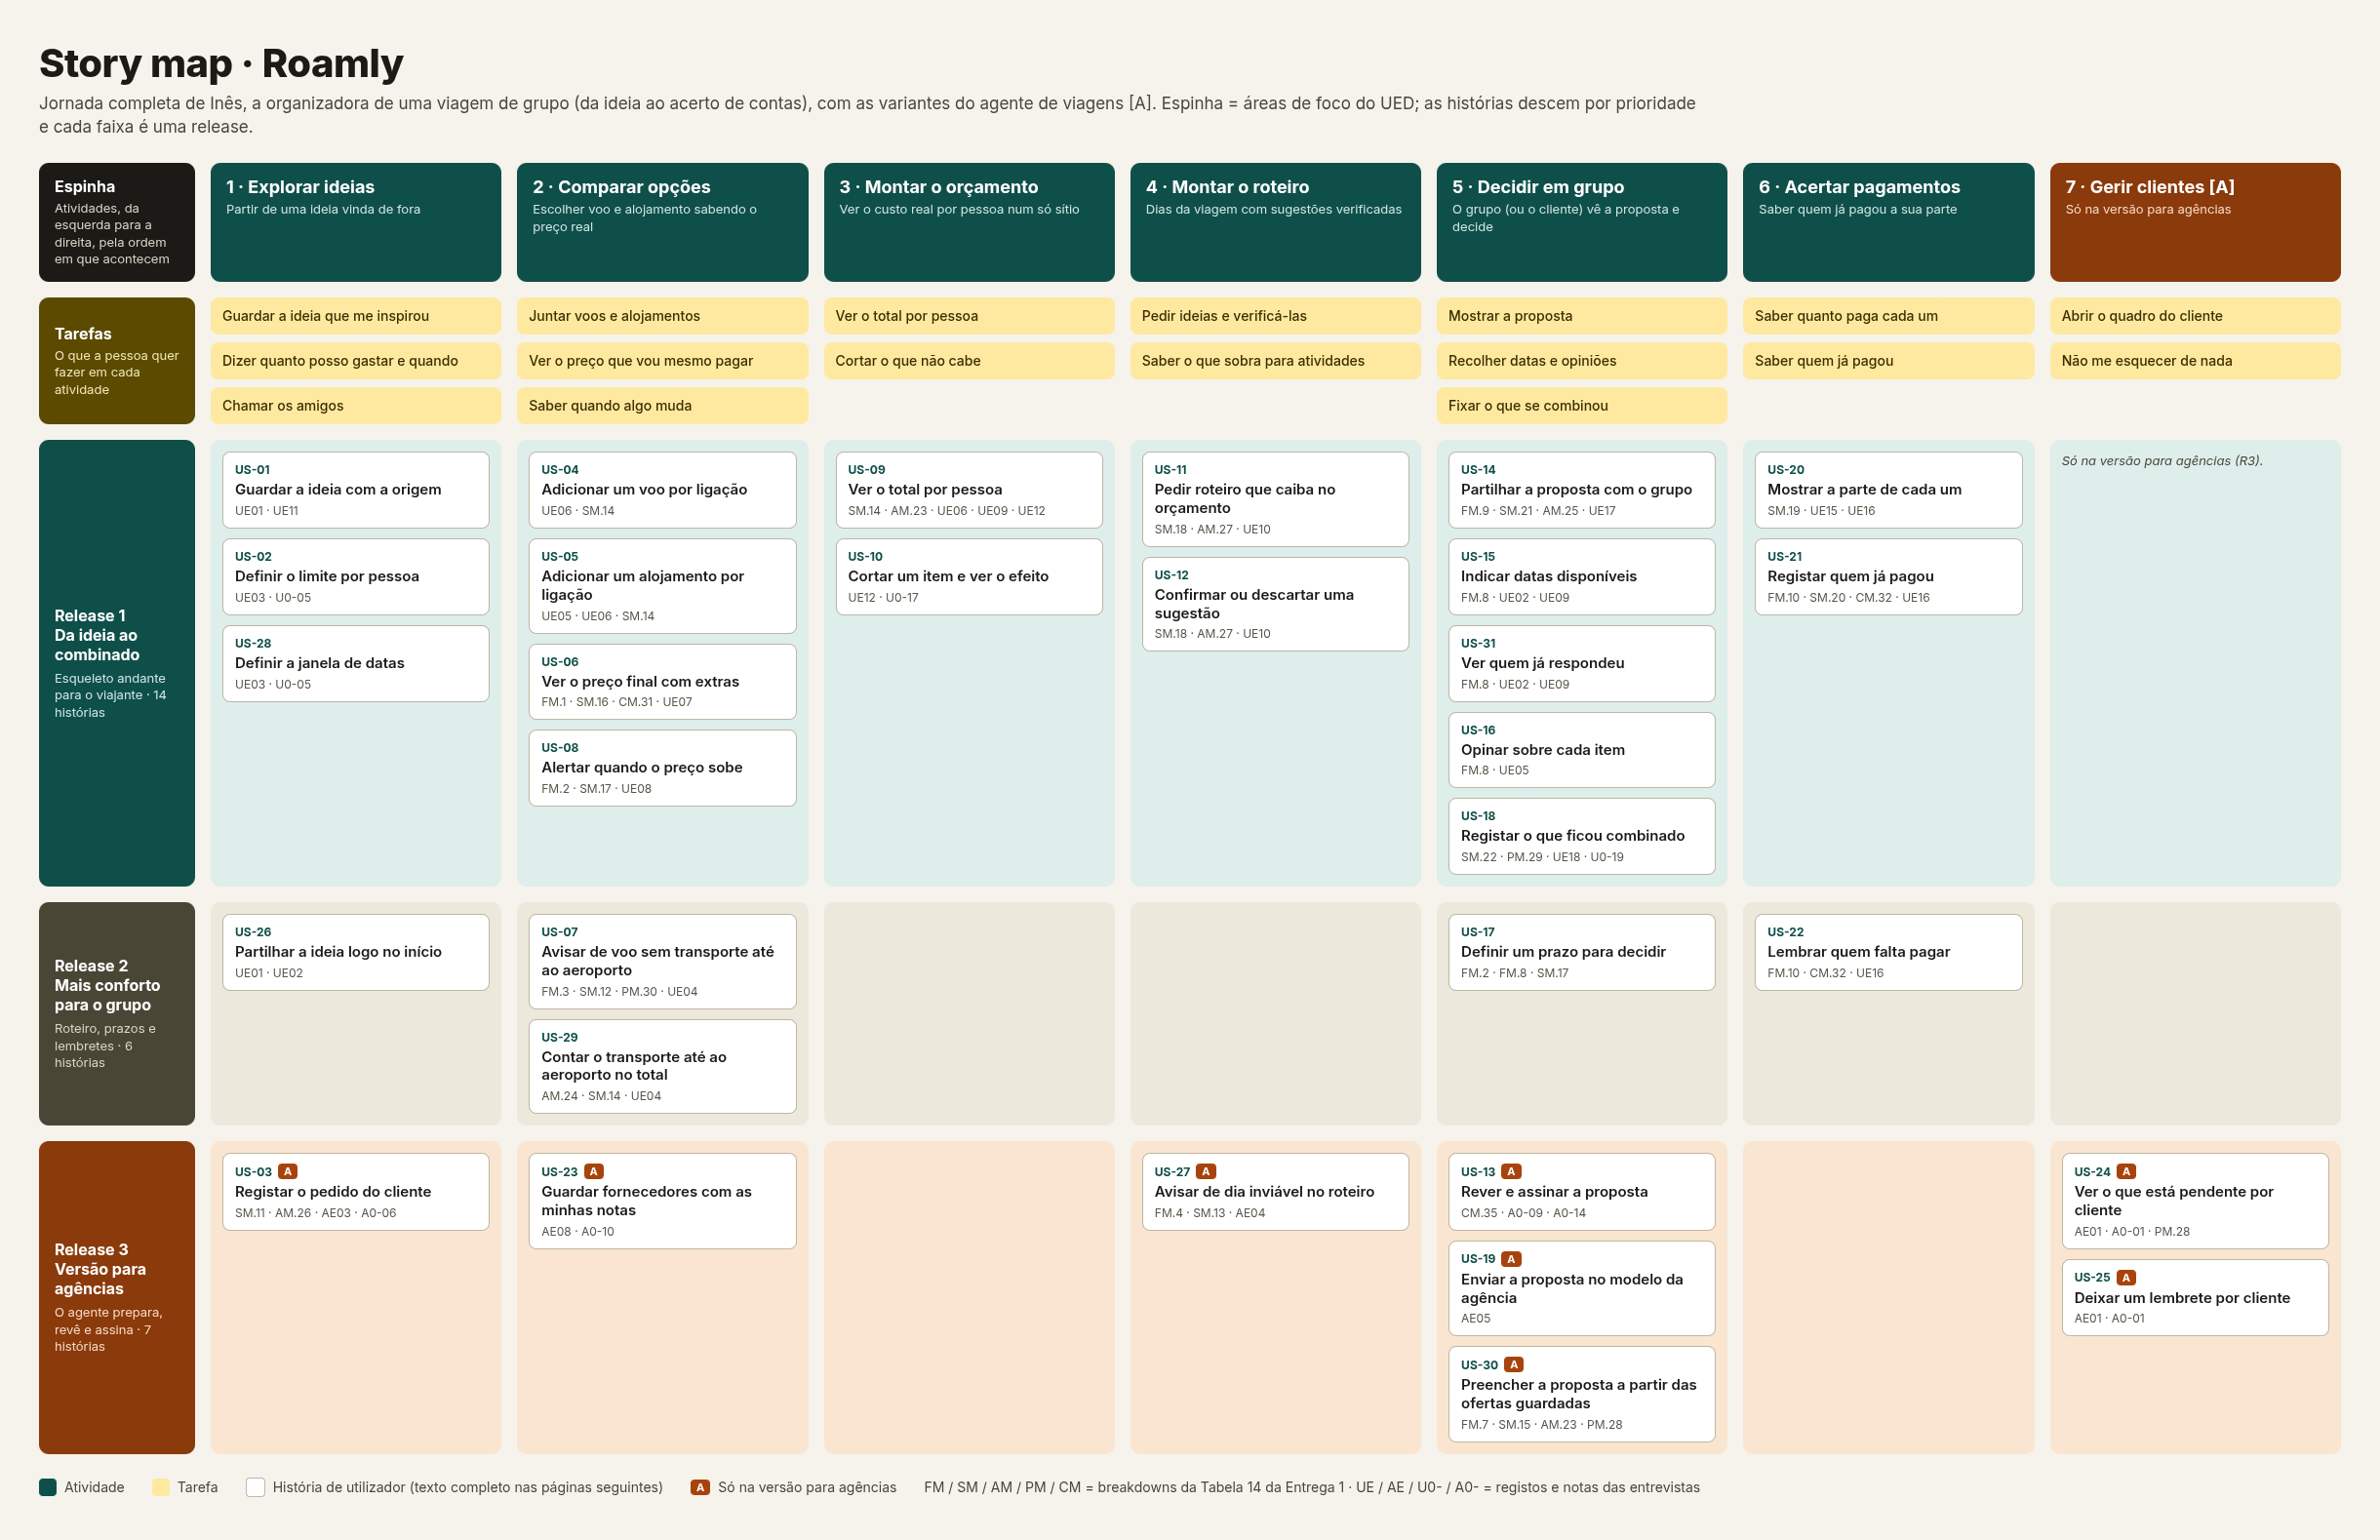
\includegraphics[width=\linewidth,height=0.8\textheight,keepaspectratio]{story_map/story_map.png}
\caption{\textit{Story map} do \projeto.}
\label{fig:storymap}
\end{figure}
\end{landscape}

% Tabela gerada a partir de ../story_map/historias_roamly.md (editar o .md e voltar a gerar)
% Pacotes necessários no preâmbulo: \usepackage{longtable,booktabs,array}
% Cole este bloco no sítio onde quer a tabela (ex.: Secção 2, Story map). [A] = só versão para agências.
{\small
\setlength{\tabcolsep}{4pt}
\begin{longtable}{@{}p{1.5cm}p{5.1cm}p{5.2cm}p{3.6cm}@{}}
\caption{Histórias de utilizador do Roamly, agrupadas por release.}\label{tab:historias}\\
\toprule \textbf{ID} & \textbf{História} & \textbf{Critérios de aceitação} & \textbf{Origem e dependências} \\ \midrule
\endfirsthead
\toprule \textbf{ID} & \textbf{História} & \textbf{Critérios de aceitação} & \textbf{Origem e dependências} \\ \midrule
\endhead
\bottomrule \endfoot
\multicolumn{4}{@{}l}{\textbf{Release 1 — Da ideia ao combinado (esqueleto andante do viajante)}} \\ \midrule
\textbf{US-01}\newline Tam. S & \textbf{Guardar a ideia com a origem.}\newline Como organizadora do grupo, quero colar a ligação de um vídeo ou escrever uma ideia de viagem, para a guardar com a origem à vista em vez de a perder entre abas e capturas de ecrã. & (1) Ao colar uma ligação, a ideia fica guardada com o endereço de origem visível.\newline (2) Se for um vídeo, o Roamly guarda-o sem o interpretar e pede-me o destino em texto. & Origem: UE01, UE11; restrição do UED (a IA só lê texto e ligações) \\ \addlinespace
\textbf{US-02}\newline Tam. S & \textbf{Definir orçamento e datas.}\newline Como organizadora, quero indicar o limite por pessoa e as datas possíveis, para que tudo o que juntar seja comparado com o que o grupo pode gastar. & (1) Guardo um limite por pessoa (ex.: 300 €) e uma janela de datas (ex.: um mês inteiro).\newline (2) O limite fica visível em todas as janelas onde aparecem preços. & Origem: UE03, U0-05; perfil U0 (300 € por pessoa) \\ \addlinespace
\textbf{US-04}\newline Tam. M & \textbf{Adicionar um voo por ligação.}\newline Como organizadora, quero colar a ligação de uma oferta de voo e ver preço, horários e condições lidos automaticamente, para não os copiar à mão para uma folha de cálculo. & (1) Com uma ligação válida, a oferta aparece no Caderno com preço por pessoa e horários, sem eu escrever nada.\newline (2) Se o Roamly não conseguir ler a página, diz-me e deixa-me preencher à mão. & Origem: FM.7, SM.15, PM.28, UE06\newline Depende de: Risco: acesso aos dados dos sites (Secção 2.6) \\ \addlinespace
\textbf{US-05}\newline Tam. M & \textbf{Adicionar um alojamento por ligação.}\newline Como organizadora, quero colar a ligação de um alojamento e ver preço por noite e condições, para o comparar com outros sem abrir um site de cada vez. & (1) A opção aparece com o preço por pessoa e noite e o total para as noites da viagem.\newline (2) Posso abrir o site original em ``Ver no site'' para confirmar a informação. & Origem: FM.7, PM.28, UE05, UE06\newline Depende de: US-04 \\ \addlinespace
\textbf{US-06}\newline Tam. M & \textbf{Ver o preço final com extras.}\newline Como organizadora, quero ver o preço final de um voo já com a bagagem de porão, para não ter surpresas na página de pagamento. & (1) A oferta mostra preço base, extras e ``Preço final''.\newline (2) Se o site não revelar os extras, aparece ``extras por confirmar'' em vez de os omitir. & Origem: FM.1, SM.16, CM.31, UE07 (bagagem +34 €)\newline Depende de: US-04 \\ \addlinespace
\textbf{US-08}\newline Tam. M & \textbf{Alertar quando o preço sobe.}\newline Como organizadora, quero ser avisada quando o preço de uma oferta guardada sobe, para decidir antes de ele subir ainda mais. & (1) O Roamly volta a ler as ligações guardadas e, se o preço subiu, a oferta mostra de quanto.\newline (2) Recebo uma notificação; o Roamly não congela preços nem faz reservas. & Origem: FM.2, SM.17, UE08 (o voo subiu 19 €)\newline Depende de: US-04, US-05 \\ \addlinespace
\textbf{US-09}\newline Tam. S & \textbf{Ver o total por pessoa.}\newline Como organizadora, quero ver num só sítio o total por pessoa das opções escolhidas, para saber se a viagem cabe no limite sem refazer contas à mão. & (1) O total atualiza-se sozinho quando um preço muda.\newline (2) Quando passa o limite, aparece um aviso junto ao total. & Origem: SM.14, AM.23, UE06, UE09, UE12 (303 $\rightarrow$ 322 $\rightarrow$ 294 €) \\ \addlinespace
\textbf{US-10}\newline Tam. S & \textbf{Cortar um item e ver o efeito.}\newline Como organizadora, quero cortar um item e ver logo o novo total, ficando o item riscado e à vista, para mostrar ao grupo o que cortei e porquê. & (1) Ao cortar, o total por pessoa recalcula-se de imediato.\newline (2) O item cortado continua visível, riscado, e posso repô-lo. & Origem: UE12 (mina de sal, 28 €), U0-17\newline Depende de: US-09 \\ \addlinespace
\textbf{US-14}\newline Tam. M & \textbf{Partilhar a proposta com o grupo.}\newline Como organizadora, quero partilhar a proposta numa ligação que os amigos veem sem abrir folhas de cálculo, para deixarem de pedir ``manda print''. & (1) Quem recebe a ligação vê itens, preços e total por pessoa sem abrir mais nada.\newline (2) A proposta partilhada reflete as alterações que eu fizer depois. & Origem: FM.9, SM.21, AM.25, UE17\newline Depende de: US-09 \\ \addlinespace
\textbf{US-15}\newline Tam. S & \textbf{Indicar datas disponíveis.}\newline Como membro do grupo, quero indicar se posso nas datas propostas ou em que outras posso, para o organizador deixar de esperar por respostas soltas. & (1) Escolho a data proposta ou indico a minha.\newline (2) A organizadora vê quem já respondeu e quem falta. & Origem: FM.8, UE02, UE09\newline Depende de: US-14 \\ \addlinespace
\textbf{US-16}\newline Tam. S & \textbf{Opinar sobre cada item.}\newline Como membro do grupo, quero marcar ``Concordo'' ou ``Prefiro outra'' em cada item da proposta, para dizer o que não aceito antes de se reservar. & (1) Cada item (voo, alojamento\ldots{}) mostra a minha resposta e a dos outros.\newline (2) A organizadora vê onde há divergência e só reserva quando todos concordam. & Origem: FM.8, UE05 (``dormitório não'')\newline Depende de: US-14 \\ \addlinespace
\textbf{US-18}\newline Tam. S & \textbf{Registar o que ficou combinado.}\newline Como organizadora, quero registar na própria proposta o que o grupo decidiu, para não ter de o passar a limpo depois de cada conversa. & (1) Escrevo o combinado na proposta e todos os membros o veem.\newline (2) O registo fica junto dos itens a que se refere. & Origem: SM.22, PM.29, UE18, U0-19\newline Depende de: US-14 \\ \addlinespace
\textbf{US-20}\newline Tam. S & \textbf{Mostrar a parte de cada um.}\newline Como organizadora, quero ver quanto cada pessoa paga antes de reservar, para pedir o valor certo e saber quanto vou adiantar. & (1) A parte de cada um é calculada a partir dos itens acordados.\newline (2) Vejo o total que terei de adiantar ao reservar. & Origem: SM.19, UE15, UE16 (98 € a cada amigo)\newline Depende de: US-09 \\ \addlinespace
\textbf{US-21}\newline Tam. S & \textbf{Registar quem já pagou.}\newline Como organizadora, quero marcar que um amigo já me pagou, para saber quem falta sem controlar de cabeça. & (1) Só eu, como organizadora, posso marcar um pagamento como feito.\newline (2) O Roamly não processa pagamentos: apenas regista. & Origem: FM.10, SM.20, CM.32, UE16\newline Depende de: US-20 \\ \addlinespace
\midrule
\multicolumn{4}{@{}l}{\textbf{Release 2 — Mais conforto para o grupo}} \\ \midrule
\textbf{US-26}\newline Tam. S & \textbf{Partilhar a ideia logo no início.}\newline Como organizadora, quero partilhar a ideia guardada com os amigos logo no início, para ver quem alinha antes de gastar tempo a pesquisar. & (1) Posso enviar a ideia guardada aos amigos a partir da janela Pesquisa.\newline (2) Os amigos veem a ideia com a origem e o limite por pessoa. & Origem: UE01, UE02; ligação 1 $\rightarrow$ 5 do UED\newline Depende de: US-01, US-02 \\ \addlinespace
\textbf{US-07}\newline Tam. M & \textbf{Avisar de voo sem transporte até ao aeroporto.}\newline Como organizadora, quero ser avisada quando um voo me obriga a chegar ao aeroporto a uma hora sem transporte, e ver o custo dessa viagem no total, para não escolher um voo que não consigo apanhar. & (1) Ao escolher um voo, aparece um aviso se não há transporte à hora necessária.\newline (2) O custo do transporte até ao aeroporto entra no total por pessoa. & Origem: FM.3, SM.12, AM.24, PM.30, UE04\newline Depende de: US-04, US-09. Risco: precisa de dados de horários de transportes (por confirmar) \\ \addlinespace
\textbf{US-11}\newline Tam. M & \textbf{Pedir um roteiro que caiba no orçamento.}\newline Como organizadora, quero pedir à IA um roteiro que caiba no que sobra do orçamento, para ter ideias de atividades baratas sem passar do limite. & (1) O Roamly mostra quanto sobra por pessoa antes de eu pedir o roteiro.\newline (2) Cada sugestão traz a fonte e o custo. & Origem: SM.18, AM.27, UE10\newline Depende de: US-09 \\ \addlinespace
\textbf{US-12}\newline Tam. S & \textbf{Confirmar ou descartar uma sugestão.}\newline Como organizadora, quero ver cada sugestão no mapa e marcá-la como confirmada ou descartada, para só contar com o que é verdade. & (1) Cada sugestão pode ser aberta no mapa.\newline (2) Fica marcada como confirmada ou descartada e o estado é visível ao grupo. & Origem: SM.18, AM.27, UE10 (confirmou 2, descartou 1)\newline Depende de: US-11 \\ \addlinespace
\textbf{US-17}\newline Tam. S & \textbf{Definir um prazo para decidir.}\newline Como organizadora, quero fixar um prazo para o grupo decidir, para as respostas não ficarem em aberto enquanto o preço sobe. & (1) O prazo aparece a todos os membros na proposta.\newline (2) Se o preço subir antes do prazo, o grupo é avisado. & Origem: FM.2, FM.8, SM.17\newline Depende de: US-08, US-14 \\ \addlinespace
\textbf{US-22}\newline Tam. S & \textbf{Lembrar quem falta pagar.}\newline Como organizadora, quero que o Roamly lembre quem ainda não me pagou, para não ter de cobrar eu a cada amigo. & (1) Quem não está marcado como pago recebe um lembrete.\newline (2) Posso decidir quando o lembrete é enviado. & Origem: FM.10, CM.32, UE16 (``só no fim do mês'')\newline Depende de: US-21 \\ \addlinespace
\midrule
\multicolumn{4}{@{}l}{\textbf{Release 3 — Versão para agências}} \\ \midrule
\textbf{US-03} [A]\newline Tam. S & \textbf{Registar o pedido do cliente.}\newline Como agente de viagens, quero registar o roteiro que o cliente traz, com o orçamento, as datas flexíveis e ``o que não abdicam'', para não perder o que o roteiro não diz. & (1) O pedido guarda o roteiro (ligação ou texto) e os três campos.\newline (2) Se faltar algum dos três, o pedido assinala-o antes de eu montar a proposta. & Origem: SM.11, AM.26, AE03, A0-06\newline Depende de: US-24 \\ \addlinespace
\textbf{US-23} [A]\newline Tam. S & \textbf{Guardar fornecedores com as minhas notas.}\newline Como agente de viagens, quero guardar fornecedores que não estão online, com as minhas notas, para os ter à mão ao montar propostas e não só no caderno. & (1) Guardo um fornecedor com notas (ex.: ``pedir quarto nos pisos de cima'').\newline (2) As opções guardadas aparecem junto das outras no Caderno. & Origem: AE08, A0-10; persona Rui \\ \addlinespace
\textbf{US-27} [A]\newline Tam. M & \textbf{Avisar de dia inviável no roteiro.}\newline Como agente de viagens, quero ser avisado quando um dia do roteiro que o cliente traz não é viável (deslocações longas, sítios fechados), para não montar uma proposta que não funciona. & (1) O aviso diz qual é o dia e a razão (ex.: duas cidades a 6 h de comboio).\newline (2) Posso ignorar o aviso e manter o dia. & Origem: FM.4, SM.13, AE04\newline Depende de: US-03 \\ \addlinespace
\textbf{US-13} [A]\newline Tam. M & \textbf{Rever e assinar a proposta.}\newline Como agente de viagens, quero rever e assinar a proposta preparada pela IA antes de o cliente a ver, para nada chegar ao cliente sem a minha validação. & (1) O cliente não vê a proposta enquanto eu não a assinar.\newline (2) Posso alterar qualquer item antes de assinar. & Origem: CM.35, A0-09, A0-14; Secção 6.2 (referida como US-13)\newline Depende de: Questão em aberto: como sabe o cliente que a proposta foi revista por uma pessoa? \\ \addlinespace
\textbf{US-19} [A]\newline Tam. M & \textbf{Enviar a proposta com o logótipo da agência.}\newline Como agente de viagens, quero enviar ao cliente a proposta com o logótipo da agência e os preços atualizados, sem copiar dados do portal, para responder depressa. & (1) A proposta sai no modelo da agência, com o logótipo.\newline (2) Os dados vêm das ofertas guardadas, não de cópia manual. & Origem: FM.7, SM.15, AE05, FM.6 (taxa de serviço)\newline Depende de: US-13 \\ \addlinespace
\textbf{US-24} [A]\newline Tam. S & \textbf{Abrir um quadro por cliente.}\newline Como agente de viagens, quero abrir ou criar um quadro por cliente e ver o que está pendente, para trabalhar num só sítio em vez de várias aplicações. & (1) Posso criar um quadro para um cliente novo.\newline (2) Cada quadro mostra os pedidos novos e as propostas por enviar. & Origem: AE01, A0-01, PM.28 \\ \addlinespace
\textbf{US-25} [A]\newline Tam. S & \textbf{Deixar um lembrete no quadro.}\newline Como agente de viagens, quero deixar um lembrete no quadro do cliente, para deixar de depender do papel autocolante no monitor. & (1) O lembrete (ex.: ``ligar ao cliente X'') fica no quadro desse cliente.\newline (2) Os lembretes pendentes aparecem junto do que está por fazer. & Origem: AE01, A0-01\newline Depende de: US-24 \\ \addlinespace
\midrule
\end{longtable}
}


%==========================================================
\section{Casos de uso}\label{sec:casosdeuso}

%----------------------------------------------------------
% Não é o diagrama de contexto do Contextual Design (nota do enunciado).
\subsection{Diagrama de contexto (nível 0)}\label{sec:contexto}

\begin{figure}[H]
\centering
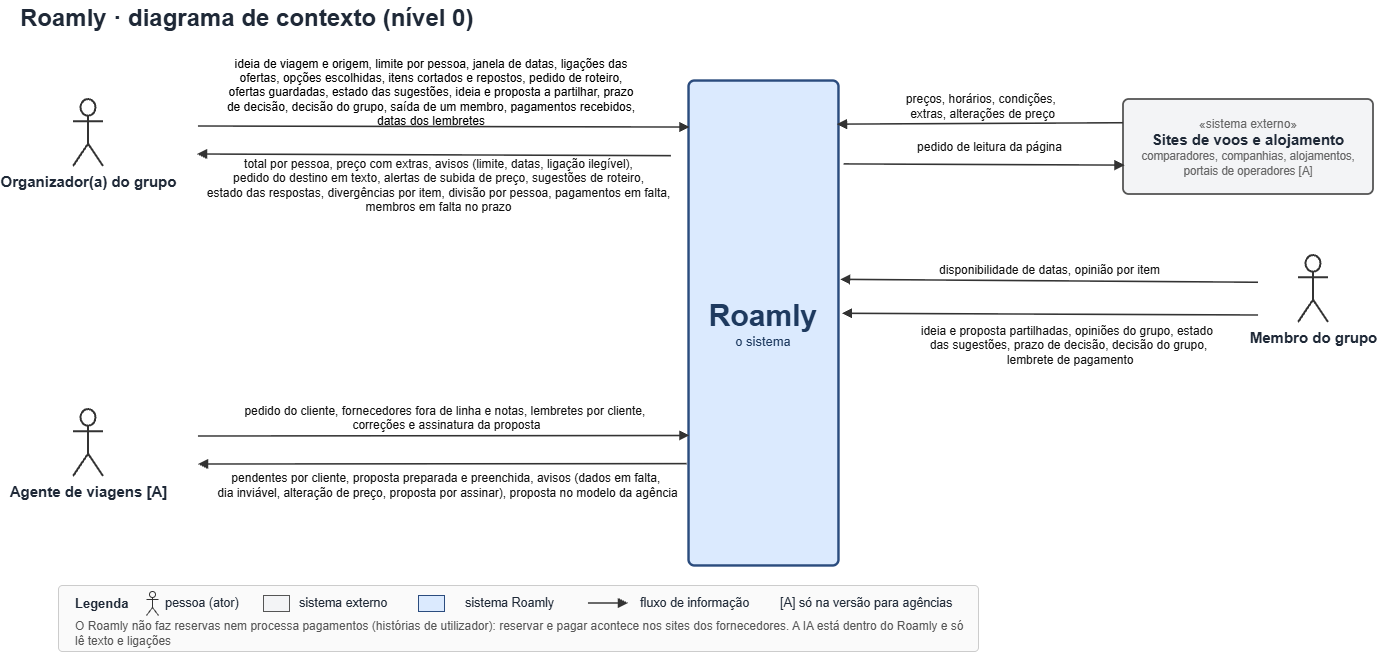
\includegraphics[width=\textwidth]{diagramas/diagrama_contexto_nivel0/Roamly-diagrama-contexto-N0.drawio.png}
\caption{Diagrama de contexto (nível 0) do \projeto.}
\label{fig:contexto}
\end{figure}


%----------------------------------------------------------
\subsection{Diagrama de casos de uso (nível 1)}\label{sec:diagrama-uc}

O diagrama da Figura~\ref{fig:diagrama-uc} mostra os casos de uso da Release~1, derivados das histórias da
Secção~\ref{sec:storymap}. O organizador do grupo é o ator principal e está ligado aos objetivos que inicia. Os membros do
grupo e os sites dos fornecedores são atores secundários: o Roamly precisa deles para cumprir o objetivo. Os sites dos
fornecedores são um sistema externo, por isso estão marcados com \guillemotleft sistema\guillemotright. Cada caso de uso indica
o seu nível de Cockburn. As relações \guillemotleft include\guillemotright{} e \guillemotleft extend\guillemotright{} mostram o
comportamento partilhado (calcular o total por pessoa) e o opcional (cortar um item, alertar a subida de preço), com os pontos
de extensão indicados nos casos base.

\begin{figure}[H]
\centering
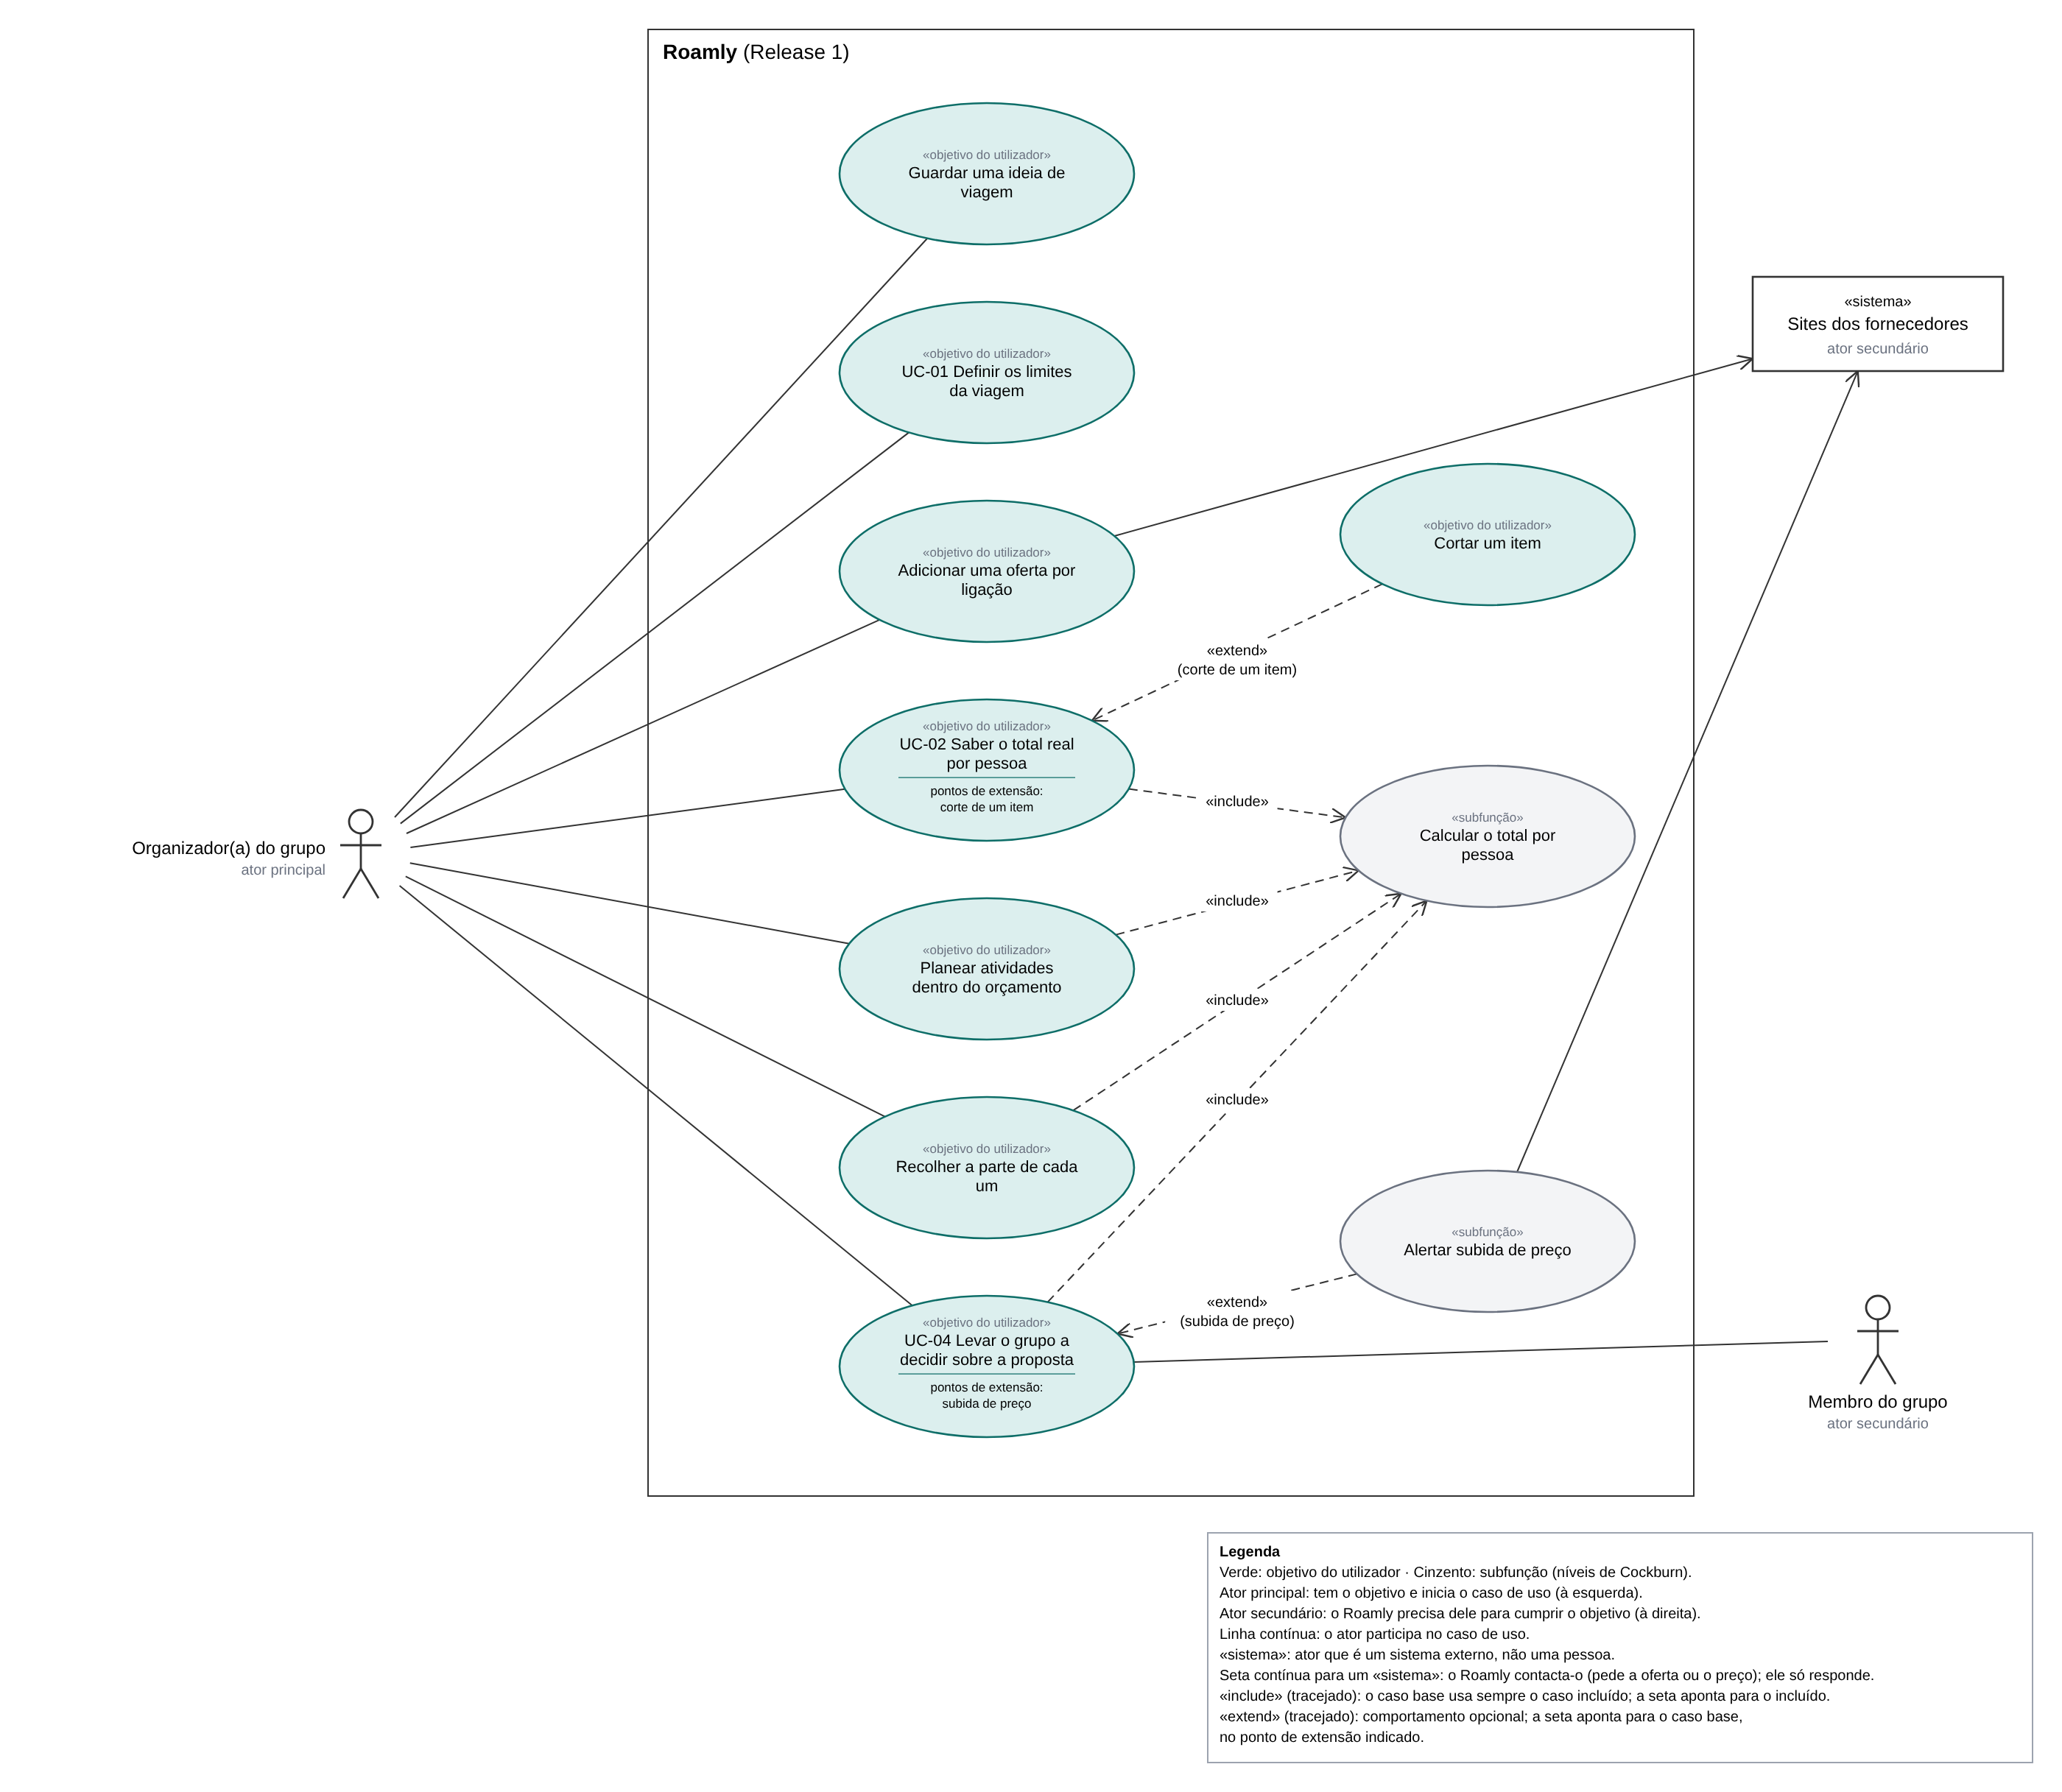
\includegraphics[width=\textwidth]{diagramas/diagrama-nivel1/use-case-diagram.png}
\caption{Diagrama de casos de uso do \projeto{} (Release 1).}
\label{fig:diagrama-uc}
\end{figure}

%----------------------------------------------------------
\subsection{Casos de uso detalhados}\label{sec:uc-detalhados}

Os três casos de uso detalhados cobrem as histórias de maior prioridade da Release~1: definir os limites da viagem (UC-01),
saber o total real por pessoa (UC-02) e levar o grupo a decidir sobre a proposta (UC-04). Seguem o modelo de Cockburn e
cada um indica as histórias, a sequência consolidada, as funções do UED e os \textit{breakdowns} em que se baseia.

% Fonte: ../casos_de_uso/corrigidos/ (os originais, gerados por IA, estão em ../casos_de_uso/)
\begingroup
\setlength{\parindent}{0pt}
\setlength{\parskip}{4pt}
\clearpage
\documentclass[11pt,a4paper]{article}
\usepackage[utf8]{inputenc}
\usepackage[T1]{fontenc}
\usepackage[portuguese]{babel}
\usepackage{lmodern}
\usepackage[margin=2.3cm]{geometry}
\usepackage{tabularx,booktabs,array,enumitem}
\usepackage[table]{xcolor}
\usepackage{textcomp}
\usepackage{hyperref}

\definecolor{roamly}{HTML}{0E6E68}
\definecolor{pendente}{HTML}{6B7280}
\hypersetup{colorlinks=true,linkcolor=roamly,urlcolor=roamly}
\newcolumntype{L}{>{\raggedright\arraybackslash}X}
\renewcommand{\arraystretch}{1.3}
\setlist{nosep,leftmargin=*}
\setlength{\parindent}{0pt}
\setlength{\parskip}{4pt}

% reference to an interview record or a breakdown (as in the report)
\newcommand{\reg}[1]{{\footnotesize\textcolor{pendente}{(#1)}}}
% use case
\newenvironment{usecase}[2]{%
  \par\medskip\noindent{\large\bfseries\color{roamly}#1: #2}\par\smallskip\small\noindent\ignorespaces}{\par\medskip}
\newcommand{\ucField}[2]{\textbf{#1} & #2 \\}

\begin{document}

\begin{usecase}{UC-01}{Definir os limites da viagem}
\textbf{Descrição breve.} Antes de procurar opções, o organizador do grupo indica quanto cada pessoa pode gastar e em que datas o grupo pode viajar. O sistema guarda estes limites na viagem e compara com eles tudo o que o organizador juntar depois. Assim, a viagem parte do orçamento e das datas do grupo, e não de um destino.\par\smallskip
\begin{tabularx}{\textwidth}{@{}>{\raggedright\arraybackslash}p{3.4cm}L@{}}
\toprule
\ucField{Ator principal}{Organizador(a) do grupo}
\ucField{Atores secundários}{Nenhum}
\ucField{Nível}{Objetivo do utilizador}
\ucField{Âmbito}{Roamly (versão base, viajante)}
\ucField{Área de foco}{1. Explorar ideias}
\ucField{Gatilho}{O grupo responde à ideia de viagem com as suas condições de preço e de datas («depende do preço; era mais fácil perto do fim de semana») \reg{UE02}.}
\ucField{Pré-condições}{Existe uma ideia de viagem guardada no Roamly («Guardar uma ideia de viagem», US-01). A viagem ainda não precisa de ter destino.}
\ucField{Garantia mínima}{O limite por pessoa e as datas já indicados ficam guardados. Nenhuma opção é comparada com um limite que o organizador não indicou.}
\ucField{Garantia de sucesso}{A viagem tem um limite por pessoa e uma janela de datas. Cada opção que o organizador juntar é comparada com eles, e o total por pessoa (UC-02) tem um limite com que ser comparado.}
\bottomrule
\end{tabularx}

\medskip
\textbf{Partes interessadas e interesses}
\begin{itemize}
  \item \textbf{Organizador(a) do grupo:} planear uma viagem barata que todo o grupo aceite, até 300\,€ por pessoa; partir do orçamento e das datas, e não do destino \reg{UE03, U0-05}; não ter de refazer tudo à mão quando uma condição muda \reg{UE09}.
  \item \textbf{Membros do grupo:} não ficarem presos a uma viagem acima do que podem pagar ou em datas em que não podem ir \reg{UE02, U0-03}.
  \item \textbf{Família (guardião financeiro):} «não gastes o que não tens» \reg{U0-12}.
\end{itemize}

\textbf{Cenário principal de sucesso}
\begin{enumerate}
  \item O organizador indica quanto cada pessoa pode gastar (p.\,ex., até 300\,€ por pessoa).
  \item O sistema guarda o limite por pessoa na viagem.
  \item O organizador indica as datas em que o grupo pode viajar.
  \item O sistema guarda a janela de datas na viagem.
\end{enumerate}

\textbf{Extensões}
\begin{itemize}[leftmargin=2.2em]
  \item[1a.] \textit{Ainda não se sabe quanto o grupo pode gastar} («depende do preço», \reg{UE02}): o organizador avança sem limite. Sempre que junta uma opção, o sistema lembra-o de que não há limite com que a comparar (US-02). Continua no passo 3.
  \item[3a.] \textit{O grupo pode ir em qualquer altura de um período} («mês inteiro», \reg{UE03, U0-05}): o organizador indica o período inteiro como janela de datas, sem destino fixo. Continua no passo 4.
  \item[*a.] \textit{As datas possíveis mudam depois de já haver opções na viagem} (o Amigo~B só pode a partir de uma sexta-feira concreta, \reg{UE09, U0-03}): o organizador indica a nova janela de datas (passo 3). O sistema volta a comparar as opções já juntas com as novas datas e avisa das que ficaram fora (US-28).
\end{itemize}

\textbf{Rastreabilidade}
\begin{itemize}
  \item \textbf{Histórias:} US-02 «Definir o limite por pessoa» (passos 1 e 2; 1a); US-28 «Definir a janela de datas» (passos 3 e 4; 3a, *a).
  \item \textbf{Sequência consolidada:} atividade 2 «Perceber o que quem viaja quer», passo «Saber o orçamento, as datas e o que não se abdica» (intenção: perceber o que quem viaja quer e até onde é flexível); atividade 3, pesquisa com datas «mês inteiro» \reg{UE03} (3a); atividade 7, «Refazer quando uma condição muda» \reg{UE09} (*a).
  \item \textbf{UED, área 1:} «Indicar o orçamento por pessoa, as datas possíveis e o que não se dispensa» (passos 1 a 4); «Pesquisar só por orçamento e datas, sem destino fixo» (3a). Ligação da área 5 para a área 1, «para refazer a pesquisa com novas datas» (*a).
  \item \textbf{Afinidade:} «Tenho orgulho em gastar menos».
  \item \textbf{\textit{Breakdowns}:} SM.11, AM.26 (ver nota 2).
  \item \textbf{Persona:} Inês.
\end{itemize}
\end{usecase}

\medskip
{\footnotesize\textbf{Notas para revisão.}
(1) O ator principal usa o nome das histórias e do diagrama de casos de uso. No modelo de fluxo consolidado, este objetivo junta o planeamento da viagem e a coordenação do grupo; nesta entrega, ambos são do organizador.
(2) Os \textit{breakdowns} da área 1 são SM.11 e AM.26: o roteiro do cliente não diz o orçamento, as datas flexíveis nem «o que não abdicam» \reg{A0-06}. São do agente e não entram neste caso de uso (versão base). A variante do agente é a US-03 [A] (Release~3).
(3) A função do UED da área 1 inclui também «o que não se dispensa». Fica fora deste caso de uso: só o agente mostra esse dado \reg{A0-06}, o caso do viajante não mostra o grupo a fixá-lo à partida, e nenhuma história da Release~1 o pede.
(4) O que acontece quando o organizador junta uma opção pertence a «Adicionar uma oferta por ligação»: o aviso de opção fora da janela de datas (US-28) é dessa altura. O aviso de total acima do limite está no UC-02 (4b).
(5) Não há atores secundários. Os membros do grupo dão as suas condições na conversa do grupo, fora do Roamly (é o gatilho, \reg{UE02}), e a família não usa o Roamly. Por isso estão nas partes interessadas, e não nos atores.\par}

\end{document}

\clearpage
\documentclass[11pt,a4paper]{article}
\usepackage[utf8]{inputenc}
\usepackage[T1]{fontenc}
\usepackage[portuguese]{babel}
\usepackage{lmodern}
\usepackage[margin=2.3cm]{geometry}
\usepackage{tabularx,booktabs,array,enumitem}
\usepackage[table]{xcolor}
\usepackage{textcomp}
\usepackage{hyperref}

\definecolor{roamly}{HTML}{0E6E68}
\definecolor{pendente}{HTML}{6B7280}
\hypersetup{colorlinks=true,linkcolor=roamly,urlcolor=roamly}
\newcolumntype{L}{>{\raggedright\arraybackslash}X}
\renewcommand{\arraystretch}{1.3}
\setlist{nosep,leftmargin=*}
\setlength{\parindent}{0pt}
\setlength{\parskip}{4pt}

% reference to an interview record or a breakdown (as in the report)
\newcommand{\reg}[1]{{\footnotesize\textcolor{pendente}{(#1)}}}
% use case
\newenvironment{usecase}[2]{%
  \par\medskip\noindent{\large\bfseries\color{roamly}#1: #2}\par\smallskip\small\noindent\ignorespaces}{\par\medskip}
\newcommand{\ucField}[2]{\textbf{#1} & #2 \\}

\begin{document}

\begin{usecase}{UC-02}{Saber o total real por pessoa}
\textbf{Descrição breve.} Depois de escolher as opções da viagem, o organizador do grupo quer saber quanto custa de facto a cada pessoa e se a viagem cabe no limite. O sistema soma num só sítio o preço das opções escolhidas, já com os extras, compara o total por pessoa com o limite da viagem e mantém-no atualizado quando um preço muda ou um item é cortado. Assim, o organizador deixa de copiar preços à mão para uma folha de cálculo e não tem surpresas na página de pagamento.\par\smallskip
\begin{tabularx}{\textwidth}{@{}>{\raggedright\arraybackslash}p{3.4cm}L@{}}
\toprule
\ucField{Ator principal}{Organizador(a) do grupo}
\ucField{Atores secundários}{Sites dos fornecedores (sistema externo): o sistema volta a ler as ofertas escolhidas para saber se o preço mudou (*a, *c)}
\ucField{Nível}{Objetivo do utilizador}
\ucField{Âmbito}{Roamly (versão base, viajante)}
\ucField{Área de foco}{3. Orçamento da viagem}
\ucField{Gatilho}{O organizador escolheu voo e alojamento e quer saber se a viagem cabe no limite por pessoa \reg{UE06}.}
\ucField{Pré-condições}{A viagem tem pelo menos um voo ou um alojamento guardado a partir da ligação da oferta, com o preço por pessoa lido da página ou preenchido à mão («Adicionar uma oferta por ligação», US-04, US-05). O limite por pessoa (UC-01) pode ainda não estar definido (extensão 4a).}
\ucField{Garantia mínima}{Nenhum custo conhecido fica fora do total. O que falta ou está por confirmar fica assinalado no total, em vez de ser omitido. Um item cortado não se perde.}
\ucField{Garantia de sucesso}{O organizador vê num só sítio o total por pessoa, com os extras, e se cabe no limite. O total fica na proposta, atualizado, pronto para o grupo decidir (UC-04).}
\bottomrule
\end{tabularx}

\medskip
\textbf{Partes interessadas e interesses}
\begin{itemize}
  \item \textbf{Organizador(a) do grupo:} saber se a viagem cabe nos 300\,€ por pessoa sem refazer as contas à mão \reg{UE06, UE09, UE12}; ter num só sítio o custo que hoje está espalhado pelo comparador, pelo transporte e pela folha de cálculo \reg{U0-07}; não ter surpresas na página de pagamento («isto ninguém diz», \reg{UE07, U0-08}).
  \item \textbf{Membros do grupo:} decidir com base no preço real («depende do preço», \reg{UE02}); perceber o que foi cortado e porquê \reg{UE12, U0-17}.
  \item \textbf{Família (guardião financeiro):} «não gastes o que não tens» \reg{U0-12}.
\end{itemize}

\textbf{Cenário principal de sucesso}
\begin{enumerate}
  \item O organizador escolhe as opções que entram na viagem: voo, alojamento e atividades.
  \item O sistema calcula o total por pessoa das opções escolhidas, já com os extras de cada oferta, como a bagagem de porão (inclui «Calcular o total por pessoa»).
  \item O sistema mostra ao organizador, num só sítio, o total por pessoa e de que é feito: o preço de cada opção e os seus extras.
  \item O sistema compara o total por pessoa com o limite da viagem (UC-01) e mostra ao organizador que a viagem cabe no limite.
  \item O sistema guarda o total por pessoa na proposta, pronto para ser partilhado com o grupo (UC-04).
\end{enumerate}

\textbf{Extensões}
\begin{itemize}[leftmargin=2.2em]
  \item[2a.] \textit{O site não revela o preço dos extras de uma oferta} (\reg{FM.1, SM.16, CM.31}): o sistema conta a oferta no total e indica que os extras estão por confirmar, em vez de os omitir (US-06). Continua no passo 3.
  \item[2b.] \textit{(Release 2, US-29) Um voo obriga a apanhar transporte até ao aeroporto} (comboio e metro, cerca de 13\,€ por sentido, \reg{UE04; AM.24, SM.14}): o custo desse transporte entra no total por pessoa. Se o custo não é conhecido, o total indica que falta esse custo. Continua no passo 3.
  \item[4a.] \textit{A viagem ainda não tem limite por pessoa} («depende do preço», \reg{UE02}; UC-01, 1a): o sistema mostra o total por pessoa sem o comparar e lembra o organizador de que não há limite com que o comparar (US-02). Continua no passo 5.
  \item[4b.] \textit{O total por pessoa passa o limite} (303\,€ para um limite de 300\,€, \reg{UE06}): o sistema avisa o organizador de que passou o limite (US-09). O organizador corta um item (*b) ou troca uma opção (área 2, «Comparar opções»), e o sistema volta ao passo 2.
  \item[*a.] \textit{O preço de uma opção escolhida muda} (o voo subiu 19\,€, \reg{UE08}), ou as datas mudam e as opções são refeitas (322\,€ depois de o Amigo~B mudar as datas, \reg{UE09}): o sistema deteta a mudança quando volta a ler a oferta no site do fornecedor, ou quando o organizador refaz as opções. Atualiza sozinho o total por pessoa (US-09) e volta a compará-lo com o limite (passo 4).
  \item[*b.] \textit{O organizador corta um item}; ponto de extensão \textit{corte de um item} («Cortar um item», US-10): o organizador corta a visita à mina de sal (28\,€, «isto é para turistas», \reg{UE12}). O sistema tira o item do total, que passa logo de 322\,€ para 294\,€, e o item continua visível como cortado, para o grupo ver o que saiu e porquê \reg{U0-17}. Se o organizador repuser o item, o total volta ao valor anterior. Continua no passo 3.
  \item[*c.] \textit{O sistema já não consegue ler uma oferta escolhida no site do fornecedor}: o total por pessoa mantém o último preço conhecido dessa oferta e indica que pode estar desatualizado (US-08). Continua no passo 3.
\end{itemize}

\textbf{Rastreabilidade}
\begin{itemize}
  \item \textbf{Histórias:} US-09 «Ver o total por pessoa» (passos 1 a 5; 4b, *a); US-06 «Ver o preço final com extras» (passos 2 e 3; 2a); US-10 «Cortar um item e ver o efeito» (*b); US-02 «Definir o limite por pessoa» (4a); US-08 «Alertar quando o preço sobe», critério 2 (*c); US-29 «Contar o transporte até ao aeroporto no total», Release~2 (2b).
  \item \textbf{Sequência consolidada:} atividade 5 «Juntar tudo numa proposta» (intenção: ter depressa uma proposta cujo total por pessoa caiba no orçamento), passos «Copiar os dados de outros sistemas para a proposta» \reg{UE06} e «Ver o custo real» \reg{UE07}; atividade 4, «Verificar a logística» \reg{UE04} (2b); atividade 7, «Cortar o que não cabe» \reg{UE12} (*b) e «Refazer quando uma condição muda» \reg{UE09} (*a).
  \item \textbf{UED, área 3:} «Somar o total por pessoa» (passos 2 e 3); «Avisar quando o total passa o orçamento por pessoa» (4, 4b); «Cortar um item e ver o efeito no total» (*b); «Atualizar o total quando um preço muda» (*a); «Incluir o transporte até ao aeroporto» (2b). Área 2: «Mostrar o preço final, já com extras como a bagagem de porão» (2, 2a); ligação da área 2 para a área 3 (4b).
  \item \textbf{Afinidade:} «Faço e refaço as contas eu mesmo/a»; «Copio à mão de um sistema para outro»; «Os extras só aparecem quando vou pagar»; «O custo de chegar ao aeroporto fica fora das minhas contas».
  \item \textbf{\textit{Breakdowns} (área 3):} SM.14 (passos 2 e 3; 2b); AM.24 (2b); FM.7, SM.15, AM.23, PM.28 (ver nota 2). Da área 2, por tocarem neste objetivo: FM.1, SM.16, CM.31 (2a).
  \item \textbf{Diagrama de casos de uso (L1):} inclui «Calcular o total por pessoa»; é estendido por «Cortar um item» no ponto de extensão \textit{corte de um item}; ator secundário: sites dos fornecedores.
  \item \textbf{Persona:} Inês.
\end{itemize}
\end{usecase}

\medskip
{\footnotesize\textbf{Notas.}
(1) Os sites dos fornecedores são ator secundário porque, nas extensões *a e *c, o sistema volta a ler as ofertas escolhidas para saber se o preço mudou. Os membros do grupo não são atores: não usam o Roamly neste caso de uso.
(2) FM.7, SM.15, AM.23 e PM.28 descrevem o agente a copiar à mão os dados do portal para a proposta \reg{AE05, A0-07}. Na versão base, o mesmo problema existe do lado do organizador, que copia à mão os preços de cada site para a folha de cálculo \reg{UE06}, e fica resolvido pelo cenário principal: o total é calculado a partir das ofertas guardadas, sem cópia. A variante do agente é a US-30 [A] (Release~3).
(3) A extensão 2b depende da US-29, que é da Release~2 e tem um \textit{spike} sobre a fonte de horários e preços de transportes; fica no caso de uso para mostrar desde já onde entra esse custo.
(4) O ator principal usa o nome das histórias e do diagrama de casos de uso. No modelo de fluxo consolidado, este objetivo é do papel \textit{Planeador da viagem}.
(5) O corte de um item é a extensão *b, e não 4c, porque pode acontecer em qualquer passo, e não só quando o total passa o limite.\par}

\end{document}

\clearpage
\documentclass[11pt,a4paper]{article}
\usepackage[utf8]{inputenc}
\usepackage[T1]{fontenc}
\usepackage[portuguese]{babel}
\usepackage{lmodern}
\usepackage[margin=2.3cm]{geometry}
\usepackage{tabularx,booktabs,array,enumitem}
\usepackage[table]{xcolor}
\usepackage{textcomp}
\usepackage{hyperref}

\definecolor{roamly}{HTML}{0E6E68}
\definecolor{pendente}{HTML}{6B7280}
\hypersetup{colorlinks=true,linkcolor=roamly,urlcolor=roamly}
\newcolumntype{L}{>{\raggedright\arraybackslash}X}
\renewcommand{\arraystretch}{1.3}
\setlist{nosep,leftmargin=*}
\setlength{\parindent}{0pt}
\setlength{\parskip}{4pt}

% reference to an interview record or a breakdown (as in the report)
\newcommand{\reg}[1]{{\footnotesize\textcolor{pendente}{(#1)}}}
% use case
\newenvironment{usecase}[2]{%
  \par\medskip\noindent{\large\bfseries\color{roamly}#1: #2}\par\smallskip\small\noindent\ignorespaces}{\par\medskip}
\newcommand{\ucField}[2]{\textbf{#1} & #2 \\}

\begin{document}

\begin{usecase}{UC-04}{Levar o grupo a decidir sobre a proposta}
\textbf{Descrição breve.} O organizador do grupo partilha a proposta de viagem com os amigos que vão. Cada membro indica em que datas pode ir e se aceita cada item, e o organizador regista o que o grupo combinou. O sistema mostra a todos a mesma proposta e o mesmo total por pessoa, mostra ao organizador quem já respondeu e onde o grupo diverge, e guarda a decisão na proposta. A seguir, o organizador pode sair do Roamly para reservar no site de cada fornecedor.\par\smallskip
\begin{tabularx}{\textwidth}{@{}>{\raggedright\arraybackslash}p{3.4cm}L@{}}
\toprule
\ucField{Ator principal}{Organizador(a) do grupo}
\ucField{Atores secundários}{Membros do grupo (indicam as suas datas e a sua opinião sobre cada item)}
\ucField{Nível}{Resumo: a decisão demora dias e faz-se em várias sessões, de pessoas diferentes \reg{UE08}}
\ucField{Âmbito}{Roamly (versão base, viajante)}
\ucField{Área de foco}{5. Decidir com o grupo ou o cliente}
\ucField{Gatilho}{A proposta cabe no limite por pessoa (UC-02) e o organizador quer a decisão do grupo antes de o preço mudar.}
\ucField{Pré-condições}{A viagem tem uma proposta com o total por pessoa (UC-02) e os seus limites (UC-01). O organizador sabe quem vai.}
\ucField{Garantia mínima}{As datas e as opiniões já dadas ficam guardadas. Todos os membros veem a mesma versão, atual, da proposta.}
\ucField{Garantia de sucesso}{O que o grupo combinou fica registado na proposta, junto dos itens a que se refere, e todos os membros o veem. O organizador sabe a resposta de cada um e pode sair do Roamly para reservar no site de cada fornecedor.}
\bottomrule
\end{tabularx}

\medskip
\textbf{Partes interessadas e interesses}
\begin{itemize}
  \item \textbf{Organizador(a) do grupo:} ter uma decisão antes de o preço subir \reg{UE08}; saber a quem insistir sem perguntar um a um \reg{UE08}; não ser o único a lembrar-se, depois de cada conversa, do que ficou combinado \reg{UE18, U0-19}.
  \item \textbf{Membros do grupo:} responder sem abrir folhas de cálculo («manda print») \reg{UE17}; dizer o que não aceitam («dormitório não») antes de se reservar alguma coisa \reg{UE05}; dizer quando podem ir \reg{UE02, UE09}.
\end{itemize}

\noindent\begin{minipage}{\textwidth}
\setlength{\parskip}{4pt}
\textbf{Cenário principal de sucesso}

Cada passo está na coluna de quem o faz. Os passos 3 e 4 são feitos por cada membro, no seu tempo.

\begin{tabularx}{\textwidth}{@{}>{\raggedleft\arraybackslash}p{0.5cm}LLL@{}}
\toprule
 & \textbf{Organizador(a) do grupo} & \textbf{Membros do grupo} & \textbf{Sistema} \\
\midrule
1. & Partilha a proposta com o grupo. & & \\
2. & & & Mostra a proposta a cada membro: itens, preços, total por pessoa e o que foi cortado e porquê. \\
3. & & Cada membro indica se pode ir nas datas propostas ou em que outras datas pode. & \\
4. & & Cada membro indica se aceita cada item. & \\
5. & & & Mostra ao organizador quem já respondeu, quem ainda falta e os itens em que os membros divergem. \\
6. & Regista na proposta o que o grupo combinou. & & \\
7. & & & Guarda a decisão na proposta e mostra-a a todos os membros, junto dos itens a que se refere. \\
\bottomrule
\end{tabularx}
\end{minipage}

\textbf{Extensões}
\begin{itemize}[leftmargin=2.2em]
  \item[2a.] \textit{Um membro não abre a proposta partilhada} («manda print», \reg{UE17; FM.9, SM.21, AM.25}): o organizador envia um resumo com o total por pessoa que se lê na própria conversa do grupo (US-14). Continua no passo 5, onde esse membro continua a aparecer em falta.
  \item[3a.] \textit{Um membro só pode ir noutras datas} (o Amigo~B só pode a partir de uma sexta-feira concreta, \reg{UE09, U0-03}): o sistema regista essas datas como alternativa às propostas (US-15) e mostra-as ao organizador junto da resposta desse membro (US-31). Se o organizador refizer a pesquisa, a janela de datas muda no UC-01 (*a) e a proposta atualizada volta a ser partilhada (passo 1).
  \item[4a.] \textit{Um membro não aceita um item} («dormitório não», \reg{UE05}): a resposta do membro fica visível ao grupo junto desse item, e o sistema mostra ao organizador em que itens há divergência (US-16). O organizador troca a opção (área 2, «Comparar opções») e o grupo vê a proposta atualizada (*a), ou mantém-no e continua no passo 6.
  \item[5a.] \textit{Os membros demoram a responder} (dois dias sem resposta, \reg{UE08; FM.8}): o organizador vê quem ainda falta (US-31) e insiste só com esses. Continua no passo 3 para esses membros.
  \item[5b.] \textit{(Release 2, US-17) O prazo fixado pelo organizador passa e falta alguém responder}: o sistema avisa o organizador de quem falta. Continua em 5a ou no passo 6.
  \item[6a.] \textit{O grupo decide ao vivo, à volta de um só telemóvel} (no café, \reg{UE18; SM.22, PM.29}): o organizador regista o combinado na proposta naquele momento (US-18). Continua no passo 7.
  \item[6b.] \textit{Há membros que ainda não responderam quando o organizador regista a decisão}: a decisão fica registada e esses membros também a veem (US-18). Continua no passo 7.
  \item[*a.] \textit{O organizador altera um item depois de partilhar a proposta}: quem abre a proposta vê a versão atualizada (US-14), com o novo total por pessoa.
  \item[*b.] \textit{O preço de uma opção sobe enquanto o grupo decide} (o voo subiu 19\,€: «malta, subiu», \reg{UE08; FM.2, SM.17}); ponto de extensão \textit{subida de preço}: o sistema avisa o organizador e os membros e mostra de quanto subiu, sem mensagens de urgência (US-08, «Alertar subida de preço»). O total por pessoa é atualizado e o grupo vê-o na proposta (*a).
\end{itemize}

\textbf{Rastreabilidade}
\begin{itemize}
  \item \textbf{Histórias:} US-14 (passos 1 e 2; 2a, *a); US-15 (passo 3; 3a); US-16 (passo 4; 4a); US-31 (passo 5; 3a, 5a); US-18 (passos 6 e 7; 6a, 6b); US-08 (*b); US-17, Release~2 (5b).
  \item \textbf{Sequência consolidada:} atividade 6 «Levar a proposta a quem decide» (intenção: conseguir uma decisão de quem viaja antes que o preço mude) e o seu \textit{breakdown} «o grupo responde devagar e o preço sobe» \reg{U0-09}; atividade 9, «Pôr o grupo a par das contas» \reg{UE17} e «Escolher o resto em conjunto e registá-lo» \reg{UE18}; atividade 7, «Refazer quando uma condição muda» \reg{UE09} (3a).
  \item \textbf{UED, área 5:} «Mostrar ao grupo a ideia e a proposta partilhadas» (passos 1 e 2); «Mostrar ao grupo o que foi cortado e porquê» (2); «Indicar as datas possíveis de cada amigo» (3); «Dar a opinião sobre cada opção» (4); «Registar o que ficou combinado» (6 e 7, 6a); «Avisar o grupo quando o preço sobe» (*b); «Definir um prazo para o grupo decidir» (5b). Ligação da área 5 para a área 1, «para refazer a pesquisa com novas datas» (3a).
  \item \textbf{Afinidade:} «Espero pelo grupo e entretanto o preço sobe»; «A proposta que partilho não chega aos meus amigos».
  \item \textbf{\textit{Breakdowns} (área 5):} FM.2, SM.17 (*b); FM.8 (5a); FM.9, SM.21, AM.25 (2a e passo 2); SM.22, PM.29 (6a).
  \item \textbf{Diagrama de casos de uso (L1):} inclui «Calcular o total por pessoa»; é estendido por «Alertar subida de preço» no ponto de extensão \textit{subida de preço}; ator secundário: membro do grupo.
  \item \textbf{Persona:} Inês.
\end{itemize}
\end{usecase}

\medskip
{\footnotesize\textbf{Notas para revisão.}
(1) O nível é resumo: a decisão demora dias \reg{UE08} e faz-se em várias sessões, de pessoas diferentes (partilhar, responder, insistir, registar).
(2) A extensão 5b depende da US-17, que é da Release~2; fica no caso de uso para mostrar desde já onde entra o prazo.
(3) Na extensão *b, o aviso chega ao organizador e aos membros, como na função do UED «Avisar o grupo quando o preço sobe», e respeita a restrição do UED «Não usar mensagens de urgência para pressionar a decisão», como a US-08.
(4) O ator principal usa o nome das histórias e do diagrama de casos de uso. No modelo de fluxo consolidado, este objetivo corresponde à coordenação do grupo, que nesta entrega é sempre do organizador.
(5) O cenário principal está em colunas porque há três participantes e os membros respondem cada um no seu tempo. O caso em que um membro não pode nas datas propostas e a proposta tem de mudar é um caminho alternativo, por isso está na extensão 3a, que volta ao passo 1.\par}

\end{document}

\endgroup
\clearpage

%----------------------------------------------------------
\subsection{Reflexão sobre um caso de uso gerado por IA}\label{sec:uc-ia}

As primeiras versões dos três casos de uso foram geradas com IA (Claude Code, com uma \textit{skill} do projeto que aplica o
método de \textit{Contextual Design} e o modelo de Cockburn). A Tabela~\ref{tab:uc-ia} lista o que estava errado, enganador ou
em falta nessas versões, e como e porquê foi corrigido.

\begingroup\small
\setlength{\tabcolsep}{4pt}
\begin{longtable}{@{}p{1.1cm}p{6.8cm}p{7.6cm}@{}}
\caption{O que mudou entre as versões geradas por IA e as versões finais dos casos de uso.}\label{tab:uc-ia}\\
\toprule
\textbf{Caso} & \textbf{Problema na versão gerada por IA} & \textbf{Correção e porquê} \\
\midrule
\endfirsthead
\multicolumn{3}{@{}l}{\footnotesize\textit{(continuação)}}\\
\toprule
\textbf{Caso} & \textbf{Problema na versão gerada por IA} & \textbf{Correção e porquê} \\
\midrule
\endhead
\bottomrule
\endfoot
UC-01 & \textit{Errado.} O passo 5 e as extensões 5a e 5b descreviam o que acontece depois, noutros casos de uso (juntar uma oferta; UC-02). A 5b repetia a 4b do UC-02. & O cenário acaba no passo 4 e uma nota diz onde ficam as extensões retiradas. Um caso de uso tem um só objetivo. \\
UC-01 & \textit{Enganador.} Uma nota dizia que o cenário «obriga» a fixar o limite e as datas, mas a extensão 1a deixa avançar sem limite. Dava também como resolvidos os SM.11 e AM.26 («o que não abdicam»), que o cenário não trata. & Nota reescrita: SM.11 e AM.26 são do agente e ficam para a US-03 [A] (Release~3). \\
UC-01 & \textit{Em falta.} A função do UED é «Indicar o orçamento por pessoa, as datas possíveis e o que não se dispensa»; a última parte desaparecia sem explicação. & Nota a justificar: só o agente mostra esse dado \reg{A0-06} e nenhuma história da Release~1 o pede. \\
UC-01 & \textit{Errado.} A pré-condição «O organizador criou a viagem no Roamly» refere uma ação que nenhum caso de uso nem história cobre. & Passou a «Existe uma ideia de viagem guardada (US-01)», o passo real anterior, coerente com o gatilho \reg{UE02}. \\
UC-01 & \textit{Em falta.} Não justificava a ausência de atores secundários. & Nota: os membros dão as suas condições na conversa do grupo, fora do Roamly, e a família não usa o Roamly; são partes interessadas, e não atores. \\
\midrule
UC-02 & \textit{Errado.} «Sem atores secundários», defendido numa nota, embora a extensão *a obrigue o sistema a voltar a ler a oferta no site do fornecedor para saber se o preço mudou. & Os sites dos fornecedores passam a ator secundário. Nova extensão *c para quando o site já não se consegue ler (US-08). \\
UC-02 & \textit{Errado e vago.} A pré-condição dizia «opção escolhida», mas o passo 1 é o organizador a escolher as opções; «opção guardada» continuava vago. & «Pelo menos um voo ou um alojamento guardado a partir da ligação da oferta, com o preço por pessoa lido da página ou preenchido à mão.» \\
UC-02 & \textit{Errado.} O corte de um item era a extensão 4c, mas pode acontecer em qualquer passo, e não só quando o total passa o limite. & Passou a *b, como o ponto de extensão do diagrama de casos de uso. \\
UC-02 & \textit{Forma.} O gatilho misturava o gatilho com a descrição do processo atual. & Ficou numa frase. \\
\midrule
UC-04 & \textit{Errado.} Nível «objetivo do utilizador», defendido numa nota, embora a decisão demore dias e se faça em várias sessões, de pessoas diferentes \reg{UE08}. & Passou a «resumo». \\
UC-04 & \textit{Inconsistente.} O aviso de subida de preço ia só para o organizador. A função do UED é «Avisar o grupo quando o preço sobe», com a restrição «Não usar mensagens de urgência». & O aviso chega ao organizador e aos membros, sem mensagens de urgência. \\
UC-04 & \textit{Errado.} A extensão 4a mandava trocar o item «no UC-02»; trocar uma opção é na área 2 do UED, «Comparar opções». & Remete para a área 2. \\
UC-04 & \textit{Legibilidade.} Cenário em lista simples, com três participantes e membros que respondem cada um no seu tempo. & Cenário em três colunas (organizador, membros, sistema), com os mesmos passos. A mudança de datas que altera a proposta fica na extensão 3a. \\
\midrule
Todos & \textit{Em falta.} O ator principal, «Organizador(a) do grupo», não é um papel do modelo de fluxo consolidado. & Mantido «Organizador(a) do grupo» em todos os artefactos, por coerência com as histórias, o diagrama e o modelo de domínio; uma nota indica a que parte do fluxo corresponde. \\
\end{longtable}
\endgroup


%==========================================================
\section{Cenários BDD}\label{sec:bdd}

Os cenários estão escritos em Gherkin, com as palavras-chave em português (\texttt{\# language: pt}), e seguem Dan
North\footnote{D.~North, «Introducing BDD», 2006, \url{https://dannorth.net/blog/introducing-bdd/}.}: cada cenário
descreve um só comportamento, com um contexto (\textit{Dado}), um único acontecimento (\textit{Quando}) e resultados que um
ator consegue observar (\textit{Então}). Usam as mesmas palavras dos casos de uso e das histórias, e o mesmo passo escreve-se
sempre da mesma maneira, para corresponder a uma só definição de passo quando os cenários forem automatizados.

Cada caso de uso tem um ficheiro \texttt{.feature}, com um cenário para o cenário principal de sucesso e um para cada
extensão tratada. As etiquetas (\texttt{@UC-04}, \texttt{@ext-3a}, \texttt{@US-15}, \texttt{@FM.8}) ligam cada cenário ao
passo ou à extensão do caso de uso, às histórias e aos \textit{breakdowns}.

%----------------------------------------------------------
\subsection{UC-04: Levar o grupo a decidir sobre a proposta}\label{sec:bdd-uc04}

A Tabela~\ref{tab:bdd-uc04} liga cada cenário ao UC-04. Ficaram de fora a extensão 5b, que é da Release~2, e as extensões
6b e *a, que não têm \textit{breakdown} associado.

\begin{table}[H]
\centering\small
\begin{tabularx}{\textwidth}{@{}L>{\raggedright\arraybackslash}p{3.1cm}>{\raggedright\arraybackslash}p{2.9cm}>{\raggedright\arraybackslash}p{2.5cm}@{}}
\toprule
\textbf{Cenário} & \textbf{Caso de uso} & \textbf{Histórias} & \textbf{\textit{Breakdowns}} \\
\midrule
Todos podem ir nas datas propostas e aceitam todos os itens & Cenário principal (passos 1--7) & US-14, US-15, US-16, US-31, US-18 & -- \\
A proposta partilhada mostra o que foi cortado & Cenário principal (passos 1 e 2) & US-14, US-10 & -- \\
Um membro não abre a proposta partilhada & Extensão 2a & US-14 & FM.9, SM.21, AM.25 \\
Um membro não pode ir nas datas propostas & Extensão 3a & US-15, US-31 & -- \\
Um membro não aceita um item & Extensão 4a & US-16 & -- \\
Os membros demoram a responder & Extensão 5a & US-31 & FM.8 \\
O grupo decide ao vivo, à volta de um só telemóvel & Extensão 6a & US-18 & SM.22, PM.29 \\
O preço de um voo sobe enquanto o grupo decide & Extensão *b & US-08 & FM.2, SM.17 \\
\bottomrule
\end{tabularx}
\caption{Rastreabilidade dos cenários BDD do UC-04.}
\label{tab:bdd-uc04}
\end{table}

% Fonte: ../bdd/UC-04-decide-with-the-group.feature (editar o .feature; o relatório acompanha)
\VerbatimInput[breaklines=true,fontsize=\footnotesize,frame=single,framesep=2mm,
  rulecolor=\color{roamly},numbers=left,numbersep=4pt]{../bdd/UC-04-decide-with-the-group.feature}

%==========================================================
\section{\textit{Domain-Driven Design}}\label{sec:ddd}

%==========================================================
\section{Reflexão sobre o uso de IA}\label{sec:reflexao}

Nas partes descritas nesta secção, a equipa idealizou primeiro cada componente à mão, a partir do relatório da Entrega~1.
Só depois usou a IA (Claude, Anthropic), com o mesmo ponto de partida, para comparar as duas versões. O objetivo não
foi substituir o trabalho da equipa, mas encontrar o que faltava em cada versão e juntar o melhor das duas, para chegar à
versão mais completa possível.

\subsection{\textit{Story map}}

Depois de idealizado o \textit{story map}, foram dados à IA o relatório da primeira entrega e os enunciados da primeira e da
segunda entregas, com o seguinte \textit{prompt}: «O ficheiro Elicitation é o enunciado da primeira entrega de um trabalho que
estou a fazer em grupo para uma cadeira de Engenharia de Software. O relatório que entregámos é o documento main.pdf. O
ficheiro Description é o enunciado da segunda entrega. A minha parte é fazer o story map. Consegues explicar-me o que é e
fazer-me um story board baseado no relatório que entregámos?»

A resposta da IA foi muito próxima do que procurávamos. Dividiu o mapa nas três \textit{releases} e propôs histórias de
utilizador curtas, escritas segundo os critérios INVEST, como pede o enunciado, mesmo sem lhe termos pedido as histórias.
Comparada com a versão da equipa, das 27 histórias propostas, 11 ficaram como estavam, 13 precisaram de pequenos ajustes e 3
tiveram de ser divididas em duas. Com a US-31, que saiu de um critério da US-15, ficaram 31 histórias.

\subsection{Histórias de utilizador}

As histórias foram depois revistas uma a uma, com a ajuda da IA, segundo os critérios INVEST e os dados da Entrega~1.
O \textit{prompt} foi apenas «review João's stories with the user-stories skill», sem dizer que as histórias tinham partido
de uma proposta da IA, para a revisão não ser enviesada. A revisão confirmou que os 61 registos e \textit{breakdowns} citados
existem, e apontou o que faltava: critérios de aceitação sem a forma \textit{Dado / quando / então} e sem caso de falha,
palavras de interface («Caderno», «quadro», «riscado»), histórias com duas capacidades e provas do agente usadas em histórias
do organizador. Também encontrou uma contradição: a US-16 dizia que o organizador «só reserva quando todos concordam», mas o
Roamly não faz reservas.

A IA propôs um plano de reescrita, mas as decisões foram da equipa: um só nome para o papel, «organizador(a) do grupo»;
histórias divididas com números novos (US-28 a US-31), sem sufixos a/b; e, em todas as histórias, a indicação de que a
reserva é feita fora do Roamly, no site de cada fornecedor. A equipa decidiu também passar a US-11 e a US-12 para a
Release~1, para esta cobrir a jornada toda. A IA concordou, mas desaconselhou mover também a US-07, porque depende de dados de
transportes que ninguém sabe ainda onde obter, e a US-07 ficou na Release~2. A numeração antiga do \textit{backlog} da
Entrega~1 deixou de ser usada, porque a IA não a conhecia e não acrescentava nada.

\subsection{Diagrama de casos de uso}

O diagrama de casos de uso foi pedido à IA a partir das histórias da Release~1, do material da cadeira (Cockburn, Gilson et
al., os \textit{slides} de UML) e de uma disposição definida pela equipa. A primeira versão não foi aceite: estava em inglês,
tinha subfunções que não tinham sido pedidas e não tinha pontos de extensão. Ao perguntarmos de onde vinham algumas regras,
percebemos que a IA apresentava decisões de desenho próprias como se fossem teoria e citava um critério que não está no material
da cadeira. A partir daí, demos-lhe os PDFs da cadeira e as decisões passaram a ser nossas: só as subfunções dadas como
exemplo, a IA do Roamly como parte do sistema, e não como ator, e os sites dos fornecedores como sistema externo. Corrigimos
também problemas visuais (linhas a cruzar elipses, texto cortado) e, depois da revisão do professor, pedimos a disposição
vertical, com o organizador ligado diretamente a cada objetivo.

\subsection{Casos de uso}

A reflexão sobre os casos de uso está na Secção~\ref{sec:uc-ia}, como pede o enunciado: a equipa reviu as primeiras versões,
com base em Cockburn e no UED, e a Tabela~\ref{tab:uc-ia} mostra o que mudou e porquê.

\subsection{Cenários BDD}

A equipa fixou primeiro as regras dos cenários, a partir de Dan North e do enunciado: um só comportamento por cenário, um só
\textit{Quando}, resultados observáveis, a linguagem dos casos de uso e etiquetas que ligam cada cenário à extensão, às
histórias e aos \textit{breakdowns}. Com essas regras e os casos de uso já corrigidos, a IA ajudou a escrever os primeiros
cenários, que a equipa reviu. Na revisão, retirámos um preço de voo que não vinha dos dados, passámos para um \textit{Dado} o
motivo que estava junto do acontecimento no \textit{Quando} e reescrevemos o cenário da extensão 3a do UC-04, que estava
confuso, para mostrar só o caso de um membro que não pode ir nas datas propostas. Como as entrevistas não dão datas exatas, as
datas de março usadas nos cenários são exemplos, iguais em todos os ficheiros.

\subsection{\textit{Domain-Driven Design}}

O modelo de domínio e os contextos delimitados também foram idealizados primeiro pela equipa. Depois, foram feitos dois
conjuntos de \textit{prompts} à IA, um para o modelo de domínio e outro para os contextos delimitados, e as respostas foram
comparadas com a versão da equipa.

\subsubsection{Modelo de domínio}

Para o modelo de domínio, a IA tinha como contexto o trabalho feito até ao \textit{story map}, e foram precisos três
\textit{prompts}. O primeiro foi: «My new task is now this: “Domain model (class-style diagram) in the ubiquitous language:
Trip, Proposal, Option (flight/stay/activity), Budget, Total per person, Group, Member/Coordinator, Vote/Opinion,
Availability, Decision, Price alert, Expense share, Payment… Derived from the artifact and sequence models”, can you do
it?» Como o \textit{prompt} estava em inglês, a resposta também veio em inglês, e o segundo \textit{prompt} serviu só para a
traduzir para português, por coerência com o resto do trabalho. O terceiro corrigiu incoerências entre a resposta e o
projeto, porque a IA ainda não conhecia as alterações que a equipa tinha feito às histórias.

Estes ajustes deveram-se ao contexto que demos à IA, e não à qualidade da resposta. A IA ajudou sobretudo nos diagramas,
que são a parte mais demorada de fazer à mão, e devolveu também o glossário que usou, sem lho termos pedido.

\subsubsection{Contextos delimitados}

Para os contextos delimitados, a IA tinha o mesmo contexto, já com as histórias atualizadas. O \textit{prompt} foi: «Tens
razão, as User stories foram alteradas pelo meu grupo e eu esqueci-me de tas dar. Aqui estão elas atualizadas. Agora, dou-te
a minha última tarefa: “At least two bounded contexts and a context map (e.g. Trip Planning \& Pricing / Group Decision /
Group Payments). Say what each owns, which terms change meaning across them (e.g. ‘Proposal’, ‘Member’), and the
relationships between them.” Quero a resposta em português».

O resultado ficou muito próximo da versão da equipa. A diferença principal foi o termo «coordenador» em vez de
«organizador». A IA disse tê-lo tirado do enunciado, mas veio do nosso próprio \textit{prompt}, que dizia «Member/Coordinator».
A lição é que a IA repete os termos que lhe damos, por isso o \textit{prompt} tem de usar a linguagem ubíqua do projeto.

%==========================================================
\section{Conclusão}\label{sec:conclusao}


\end{document}
